\documentclass[12pt]{article}
\usepackage{amsmath}
\usepackage{graphicx}
\usepackage{subcaption}
\usepackage{hyperref}
\usepackage{url}
\usepackage{booktabs}
\usepackage{placeins}
\usepackage{pdflscape}
\usepackage{multirow}
\usepackage{color}
\usepackage[utf8]{inputenc}

% The following parameters seem to provide a reasonable page setup.
\topmargin 0.0cm
\oddsidemargin 0.2cm
\textwidth 16cm 
\textheight 21cm
\footskip 1.0cm

% Include your paper's title, authors and date here
\title{PHY 982 Homework 3}
\author{John Ash, Mengzhi Chen, Tong Li, Jason Surbrook}
\date{March 22, 2018}

%%%%%%%%%%%%%%%%% END OF PREAMBLE %%%%%%%%%%%%%%%%

\begin{document}
\maketitle

\section{Choice of beam energies and potentials} \label{part1}
	The $^{12}$C(d, p)$^{13}$C reaction is discussed in this work. 
	The Coulomb barrier between $^{12}$C and deutron is about 2.03 MeV.
	Then, two deuteron beam energies are studied, one is 2.84 MeV near the Coulomb barrier; another one is 4.51 MeV which is about 2 times higher than the barrier .
	
	As mentioned in Ref. \cite{PhysRev.101.209}, at both energies we choose the angular distributions should be explained by assuming small amplitudes for compound nucleus formation interfering with large stripping amplitudes. 
	Therefore our calculations using FRESCO may not yield satisfying agreement with experiment.
	
	Optical potentials are needed that described the incoming and outgoing distorted waves.  
	These are interactions between the following pairs: ($^{12}$C, d) \cite{PhysRevC.73.054605}, ($^{12}$C, p) \cite{PTCOG} and ($^{13}$C, p). 
	For the potential of ($^{13}$C, p), we cannot find an appropriate one in the energy range we study, 
	so we use the potential of ($^{12}$C, p) instead. 
	For the deuteron wavefunction, the binding for the proton and neutron is described by a simple Gaussian potential 
	\begin{equation}
		V_{np}(r)=-72.15e^{-(r/1.484)^2}.
	\end{equation}
	which reproduces a bound s-state at 2.2 MeV.
	
	The neutron that is transferred in the reaction is expected to occupy a $1p_{1/2}$ orbit with an experimental single-particle binding energy of 4.946 MeV. 
	The FRESCO calculation dynamically adjusts the Woods-Saxon depth for $^{13}$C to reproduce this energy.
	
	
\section{Results of DWBA post-form calculations}

\begin{figure}[t]
	\centering
	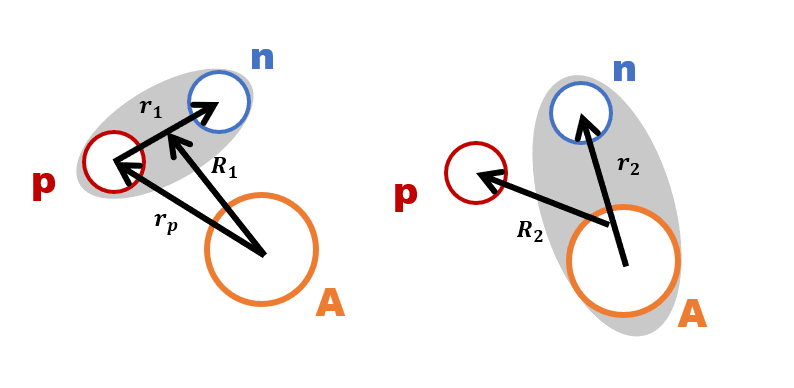
\includegraphics[width=0.80\textwidth]{transfer.png}
	\caption{Coordinates used in one neutron transfer reaction. }
	\label{fig:transfer}
\end{figure}
In a transfer reaction A(d,p)B showed in Fig. \ref{fig:transfer}, by introduction the auxiliary potential $U_f(R_2)$, the transfer T-matrix has a formula \cite{thompson2009nuclear}
\begin{equation}
	T_{post}=<\phi_{nA}\chi_{pB}^{(-)}\left|V_{np}(r_1)+U_{pA}(r_p)-U_f(R_2)\right|\Psi_1^+(\vec{r}_1,\vec{R}_1)>,
\end{equation}
where $\phi_{nA}$ and $\chi_{pB}$ are bound states wave-functions. 
Under DWBA approximation, it becomes
\begin{equation}\label{tpost}
	T_{post}^{DWBA}=<\phi_{nA}\chi_{pB}^{(-)}\left|V_{np}(r_1)+U_{pA}(r_p)-U_f(R_2)\right|\phi_{np}\chi_{dA}>.
\end{equation}
Besides that, we still need information for the auxiliary potential $U_f(R_2)$. 
It's usually chosen as $U_{pB}(R_2)$ fitted from elastic scattering.
We name $V_{np}(r_1)$ as binding potential and the rest two remnants.

Here are three different handling methods we used in our calculations.
\begin{enumerate}
\item Zero range approximation (ZRA): Remnants are neglected; $V_{np}(r_1)$ is considered as a local interaction with strength $D_0$.
	Correspondingly, the T-matrix becomes
	\begin{equation}
		T_{post}^{ZR-DWBA}=D_0<\phi_{nA}(R_1)\chi_{pB}^{(-)}| \chi_{dA}(R_1)>
	\end{equation}
	It now relies on $R_1$ only which simplifies calculation.
	\item First order DWBA without or with remnant: The former abandons the remnants but latter keeps, as well as the nonlocality of $V_{np}(r_1)$ is preserved in both.
\end{enumerate}

The results together with experimental data are presented in figures (need to be supplemented). 
We can see ZRA gives result deviates most from experiment because it applies the roughest approximation.
DWBA with or without remnants yield close results.
This makes sense because $U_{pA}$ and $U_{pB}$ are so similar that they almost cancel each other in Eq. \ref{tpost}.
But looking closer, we find the one with remnants is more contiguous to experiment.
\section{Results of prior-form DWBA calculations}
To be filled by Tong. 
\section{Extraction of spectroscopic factor}
As is normal, the spectroscopic factor is extracted by comparing the theory to the data at the first peak in the angular distribution
\cite{PhysRevC.69.064313}, as we expect that the reaction is mostly direct at the forward angle. 
The spectroscopic factors at beam energies 2.84 MeV and 4.51 MeV are given in Table \ref{tab:spec}. 
The angle of first peak $\theta_{p}$ and corresponding differential cross section $\sigma^{\mathrm{DWBA}}$ is given by the first-order DWBA calculations in post form with finite-range interactions and full complex remnant (see Sec. \ref{sec:post}). 
$\sigma^{\mathrm{exp}}$ is obtained by spline interpolation of experimental data. 
The spectroscopic factors we extract are energy-dependent. 
Ref. \cite{PhysRev.101.209} shows that, for this reaction, there is a small but considerable contribution from compound nuclear formation for the low-energy case, which explains the energy dependency of the spectroscopic factor. 
\begin{table}[bt]
	\centering
	\caption{Spectroscopic factors $S$ extracted from $^{12}$C(d, p)$^{13}$C. 
	$\theta_p$ is the angle of the first peak, and $\sigma^{\mathrm{exp}}$ and $\sigma^{\mathrm{DWBA}}$ are corresponding differential cross sections obtained from experimental data and post-form DWBA calculation, respectively. }
	\label{tab:spec}
	\begin{tabular}{ccc}
		\hline
		\hline
		Beam energy (MeV)                  & 2.84 & 4.51 \\
		\hline
		$\theta_p$ (degree)                &  31 & 25 \\
		$\sigma^{\mathrm{exp}}$ (mb/sr)    &  18.49 & 11.57 \\
		$\sigma^{\mathrm{DWBA}}$ (mb/sr)   &  43.14 & 56.40 \\
		$S=\sigma^{\mathrm{exp}}/\sigma^{\mathrm{DWBA}}$ & 0.4286  & 0.2051 \\
		\hline
		\hline
	\end{tabular}
\end{table}

\bibliographystyle{unsrt}
\bibliography{references}
\end{document}